\section{Datasets}
The application is based on two different datasets, namely LinkedGeoData and Dbpedia. It was decided to work with both datasets separately, due to the fact that LinkedGeoData is already very detailed and most data of Dbpedia is already in the other dataset. Having to different datasets allows the user to compare the results and can also give hints how accurate Dbpedia actually is. 

To get the data from LinkedGeoData, different approaches where tried. The first approach was to download all the data and use it offline. This soon appeared to be not sophisticating, because of multiple reasons. On the first hand the dataset is split, based on the main categories Amenity, SportThings, HistoricalThings, etc, with each subdataset having a large size and in case that you want to use all the data more than 40 datasets have to be loaded. On the other hand loading single datasets into a model when starting the application takes very long. Small datasets, for example all MilitaryThings need only a few seconds to be loaded, but others as for example HistoricThings need approximately one hour. As this is not feasible, to load every time that a user starts a request, it was decided to look for other ways to load the data. The most easiest way was to directly use the sparql endpoint of LinkedGeoData, which can be simply used in Jena. The used query can be found in \ref{fig:sparqlLGD}. 

\begin{figure}
	\centering
	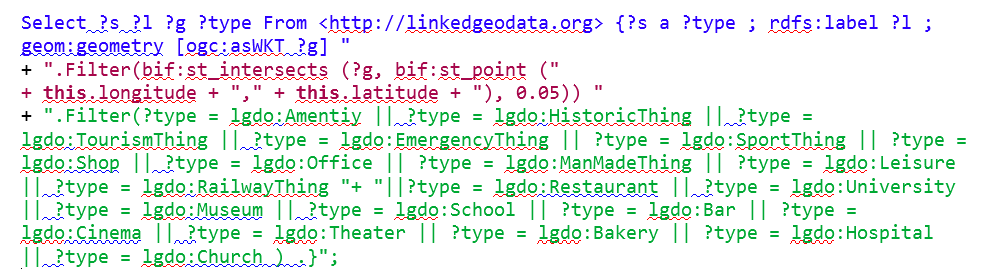
\includegraphics[scale=0.7]{./content/sparqlLGD.png}
	\caption{Sparql query to select all data of LinkedGeoData}\label{fig:sparqlLGD}
\end{figure}

The query consists of three parts which are differently colored. The blue part selects the values of the needed variables, while the red and the green part show two different filters. The first filter is used to not read the data of the whole world, but only in a given region. The region that should be used is defined by the user and then used by this.latitude and this.longitude. Using st\_intersects makes it possible to get all points that are in a specified radius around a given point. It was decided to use a 50km radius around the point that the user chose. 

In the first version of the application only the location filter was used. That allowed us to use all existing categories, what would have made the clustering very dynamic. But as there are many different categories, also some very general and thus for our use case uninteresting ones, the time to get all triples was too long. The requests were interrupted after 15 minutes waiting time, but in our opinion even a minute waiting time is not acceptable for the application. 

Due to these experiences the second filter was introduced, this time filtering the categories. Because of the separation of the dataset based on the main categories, as it is done for the download, we are already aware of the main categories which are also represented in the filter. Furthermore some more specialized categories, like museum and university are added, as they are more interesting for the clustering. Having the second filter the request needs only a few seconds, what makes the application usable.

To get the data of Dbpedia, the corresponding sparql endpoint was directly used. The query is shown in \ref{fig:sparqlDbpedia}. It is similar to the one used for LinkedGeoData, except a third filter was added, due to the fact that Dbpedia allows to have multiple labels for each resource with different language tags. Without using the language filter, there would be multiple instances for each class, one per label. Using the filter makes it sure that only the english label is used for the application and thus only one instance is created, as expected. Having multiple labels was not experienced using LinkedGeoData, that’s why the filter is not in the first query. Basically the same information was selected, except the longitude and latitude are read separately, as this worked better with the location filter. The filter on the categories has been modified, to filter the categories that are attached to a Dbpedia resource. The general idea of the types has not changed, as it is also possible to look for museums and universities, but the URIs are different. 

\begin{figure}
	\centering
	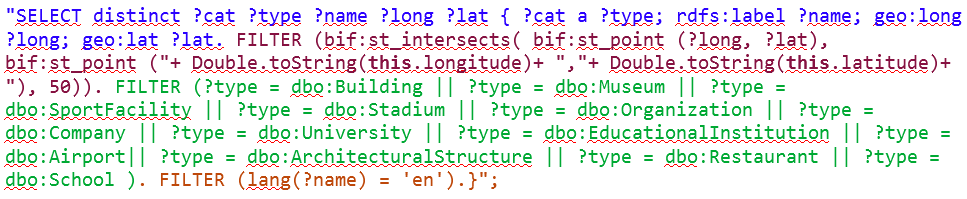
\includegraphics[scale=0.7]{./content/sparqlDbpedia.png}
	\caption{Sparql query to select all data of Dbpedia}\label{fig:sparqlDbpedia}
\end{figure}

While exploring the different resources of Dbpedia manually, one major issue for the application was found. Not all points of interest that can be found in Dbpedia have information about their location. These points can therefore not be used for the clustering and falsify the result comapared to LinkedGeoData.